\documentclass[12pt,a4paper]{article}
\usepackage{graphicx}
\usepackage[czech]{babel}
\usepackage[utf8]{inputenc}
\usepackage{titling}
\usepackage{pdfpages}
\usepackage[nopar]{lipsum}
\usepackage{mathtools}
\usepackage{multirow}
\usepackage{caption}
\usepackage{float}
\usepackage{enumitem}
\usepackage{listings}
\usepackage{amsmath}
\usepackage{amssymb}
\usepackage[left=25mm,right=25mm,top=30mm,bottom=20mm]{geometry}
\bibliography{clanky}
\bibliographystyle{abbrv}




\begin{document}
\title{SLAM\\rešerše}
\author{Jakub Kratochvíl}
\date{Akademický rok 2017/2018}
\begin{titlepage}
\begin{center}

\includegraphics[scale=0.5]{logo_zcu}\\
\vspace{5cm}
\begin{Large}
\textbf{\thetitle}\\
\end{Large}
\vspace{3cm}
\theauthor\\
\vspace{5cm}
\thedate
\end{center}
\end{titlepage}
\newpage
		
		
\tableofcontents
\newpage
\fontsize{12pt}{18pt}\selectfont


\section{Úvod}
SLAM je zkratka pro simultánní lokalizaci a mapování, jeden ze základních problémů autonomních robotů. Jeho řešením by měl být robot, schopný na neznámém místě v neznámém prostředí vytvořit mapu tohoto prostředí a zároveň se v ní sám během pohybu lokalizovat.

Do povědomí se SLAM dostal v roce 1986 na konferenci IEEE Robotics and Automation, která se konala v San Francisku v Kalifornii. V tomto období se v robotice a umělé inteligenci začaly objevovat metody založené na pravděpodobnostních principech a tak vyvstala otázka možnosti použití odhadových metod na mapovací a lokalizační problémy. Po následujících diskuzích se problém ukázal jako velice zajímavý a konzistentní pravděpodobnostní mapování stalo jedním ze základních problémů a výzev robotiky.

Aplikací SLAM můžeme najít mnoho, počínaje autonomním domácím vysavačem nebo sekačkou na trávu přes robotický průzkum opuštěných nebo člověku nebezpečných prostor, navigaci ponorek kolem podmořských přírodních překážek, řízení bezpilotních letounů a dronů až po v poslední době hodně diskutované samořídící automobily nebo dokonce planetární rovery brázdící povrch Marsu.

\textbf{TODO: předpokládané výsledky této práce}


\newpage
\section{SLAM}
SLAM je problém týkající se otázky, zda je možné najít polohu nějakého zařízení vzhledem k jeho okolí a současně mapovat strukturu prostředí.

Landmarky nebo také majáky jsou nezaměnitelné a snadno rozpoznatelné orientační body v prostředí, které mohou být v některých aplikacích dopředu známy. Například autonomní vozík pohybující se ve výrobní hale může mít předem nadefinovanou mapu landmarků. Nebo robot pro práci pod širým nebem používající pro svou orientaci GNSS (globální družicový polohový systém). V takových případech, kdy lze stroj lokalizovat vzhledem ke známým bodům, nemusí být SLAM vyžadován. Ovšem v husté zástavbě, v podzemí a uvnitř budov je použití GNSS omezené nebo úplně nemožné. V neznámém prostředí zase nelze využít předem připravenou mapu a přichází nutnost použití jiného řešení, kterým bývá nejčastěji právě SLAM. Navíc v mnoha vojenských i civilních aplikacích není cílem lokalizace, ale právě robotem vytvořená mapa, kterou poté dále zpracovává lidský operátor.

Další z impulzů vývoje simultánní lokalizace a mapování byl špatný odhad pohybu získaný z odometrie kol, čímž se rozumí například počet otáček, úhel natočení apod. Tento odhad se navíc s ujetou vzdáleností zhoršuje (tzv. drift) a tím znemožňoval použití pro správnou a přesnou lokalizaci i tvorbu mapy. Nicméně dnešní algoritmy dokáží snížit drift na přijatelnou hodnotu 0,5\% a méně, takže v tomto ohledu není nutno využívat SLAM. \\ V čem je ale stále nenahraditelný, je schopnost tzv. uzavírání smyček. Při použití dat pouze z odometrie robot vnímá svět jako "nekonečný koridor", ve kterém neustále zkoumá nové oblasti (obr.1 vlevo). SLAM ale dokáže robotem vytvořenou smyčku uzavřít, protože porovná aktuální landmarky s těmi dříve objevenými a tím dokáže správně porozumět topologii prostředí a v mapě určit, že tyto dvě chodby se protínají (obr.1 vpravo).

\begin{figure}[H]
\centering
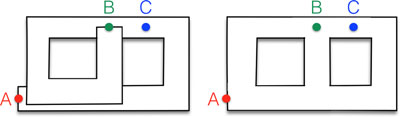
\includegraphics[scale=1]{Obr1} 
\caption{Levá mapa je vytvořená pomocí odometrie a znázorňuje jeden dlouhý koridor od bodu A do B. Body, které jsou ve skutečnosti blízko (B a C) mohou být podle této mapy libovolně daleko. Pravá mapa je vytvořená pomocí SLAM s využití uzavírání smyček, kde je znázorněná správná topologie prostředí, neboť robot správně našel "zkratku" mezi dvěma koridory.}
\end{figure}


\newpage
SLAM je ze své podstaty problém typu slepice-vejce a je tedy do značné míry netriviální. Robot pro svoji lokalizaci potřebuje mapu terénu, avšak k sestavení mapy musí znát svou vlastní polohu. Ovšem existují algoritmy, které, i přes tento rozpor, uspokojivě fungují a nasnadě je tedy otázka "Je SLAM vyřešen?". Ano i ne, otázku je nutno položit pro konkrétní konfiguraci robota, prostředí a požadavků, kde může figurovat mnoho kombinací, např. z následujících možností.
\begin{itemize}
\item Robot: dynamika, maximální rychlost, dostupné senzory, výpočetní výkon
\item Prostředí: 2D/3D, přírodní/umělé, přítomnost dynamických prvků, množství a typ landmarků, množství symetrie
\item Požadavky: přesnost odhadu stavu robota, přesnost a typ mapy, míra úspěšnosti, latence odhadu, maximální velikost mapované oblasti...
\end{itemize}
Například mapování vnitřního 2D prostředí s robotem vybaveným snímačem kol a laserovým senzorem s dostatečnou přesností a robustností lze považovat z velké části za vyřešené. Na druhou stranu další kombinace robot/prostředí/požadavky si stále zaslouží velké množství výzkumu. Aktuální algoritmy mohou snadno selhat, jestliže je pohyb robota nebo prostředí příliš náročný.


\section{Pravděpodobnostní definice}
Uvažujme mobilního robota, který projíždí neznámým prostředím a pomocí senzorů na sobě umístěných pořizuje relativní pozorování okolních landmarků (obr.2)

\begin{figure}[H]
\centering
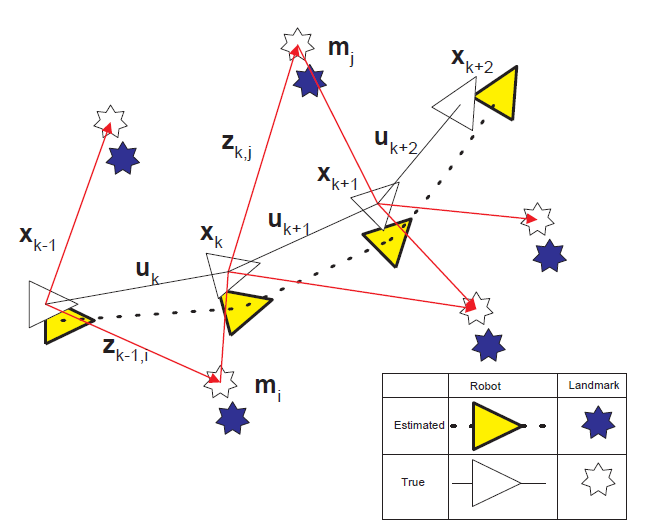
\includegraphics[scale=0.6]{Obr2}
\caption{Skutečné umístění landmarků ani robota není nikdy známo, jen jejich vzájemná poloha.}
\end{figure}

V okamžiku \textit{k} jsou definovány následující veličiny a soubory hodnot:
\begin{itemize}
\item \textbf{x}$_k$; \textbf{X}$_{0:k}=\lbrace \text{x}_0, \text{x}_1,\cdots, \text{x}_k\rbrace = \lbrace \textbf{X}_{0:k-1}, \textbf{x}_k \rbrace$:  
Stavový vektor popisující polohu a orientaci robota, respektive  historii všech stavových vektorů.
\item \textbf{u}$_k$; \textbf{U}$_{0:k}=\lbrace \text{u}_1, \text{u}_2,\cdots, \text{u}_k\rbrace = \lbrace \textbf{U}_{0:k-1}, \textbf{u}_k \rbrace$: 
Vektor řízení použitý v čase \textit{k}-1 pro dosažení stavu x$_k$ v čase \textit{k}, resp. historie vektorů řízení.
\item \textbf{m}$_i$; $\textbf{m}=\lbrace \text{m}_1, \text{m}_2,\cdots, \text{m}_n\rbrace$: 
Vektor popisující polohu i-tého landmarku, resp. vektor popisující polohy všech landmarků.
\item \textbf{z}$_{ik}$; \textbf{Z}$_{0:k}=\lbrace \text{z}_1, \text{z}_2,\cdots, \text{z}_k\rbrace = \lbrace \textbf{Z}_{0:k-1}, \textbf{z}_k \rbrace$: 
Pozorování o poloze i-tého landmarku získané z robota, resp. soubor všech pozorování.
\end{itemize}

Pro vyřešení problému musíme najít sdruženou posteriorní hustotu pravděpodobnosti landmarků \textbf{m} a stavů robota x$_k$ pro všechny časy $k$.

\begin{eqnarray}
P(\textbf{x}_k, \textbf{m} \,|\, \textbf{Z}_{0:k}, \textbf{U}_{0:k}, \textbf{x}_0)
\end{eqnarray}

Vhodné řešení nabízí rekurzivní algoritmus, kdy hustotu pravděpodobnosti v čase $k$ vypočteme pomocí hustoty v čase $k-1$, řízení u$_k$ a pozorování z$_k$.

\begin{eqnarray}
P(\textbf{x}_{k-1}, \textbf{m} \,|\, \textbf{Z}_{0:k-1}, \textbf{U}_{0:k-1})
\end{eqnarray}

Tento výpočet vyžaduje definování modelu pozorování a pohybového modelu.

\begin{enumerate}
\item \textbf{Model pozorování} popisuje s jakou pravděpodobností získáme pozorování z$_k$, pokud známe polohu robota i landmarků.
\begin{eqnarray}
P(\textbf{z}_k \,|\, \textbf{x}_k, \textbf{m})
\end{eqnarray}
\item \textbf{Pohybový model} popisuje s jakou pravděpodobností se robot nachází ve stavu x$_k$, pokud známe předchozí stav x$_{k-1}$ a aplikované řízení u$_k$.
\begin{eqnarray}
P(\textbf{x}_k \,|\, \textbf{x}_{k-1}, \textbf{u}_k)
\end{eqnarray}
\end{enumerate}

Stavový přechod pohybového modelu je Markovský proces, neboť stav x$_k$ závisí pouze na předchozím stavu x$_{k-1}$ a aplikovaném řízení u$_k$ a je nezávislý na pozorováních i mapě. SLAM algoritmus je nyní implementován ve standardní dvoustupňové (predikce-korekce) rekurzivní formě.

\newpage

\begin{enumerate}
\item \textbf{Predikce} 
\begin{eqnarray}
P(\textbf{x}_k, \textbf{m} \,|\, \textbf{Z}_{0:k-1}, \textbf{U}_{0:k}, \textbf{x}_0) \: = \: \int P(\textbf{x}_k \,|\, \textbf{x}_{k-1}, \textbf{u}_k) \: \times \: P(\textbf{x}_{k-1}, \textbf{m} \,|\, \textbf{Z}_{0:k-1}, \textbf{U}_{0:k-1}, \textbf{x}_0) d\textbf{x}_{k-1}  
\end{eqnarray}
\item \textbf{Korekce}
\begin{eqnarray}
P(\textbf{x}_k, \textbf{m} \,|\, \textbf{Z}_{0:k}, \textbf{U}_{0:k}, \textbf{x}_0) \: = \: \frac{P(\textbf{z}_k \,|\, \textbf{x}_k, \textbf{m}) P(\textbf{x}_k, \textbf{m} \,|\, \textbf{Z}_{0:k-1, \textbf{U}_{0:k}, \textbf{x}_0})}{P(\textbf{z}_k \,|\, \textbf{Z}_{0:k-1}, \textbf{U}_{0:k})}
\end{eqnarray}
\end{enumerate}

Rovnice (5) a (6) poskytují rekurzivní postup pro výpočet hustoty pravděpodobnosti $P$(\textbf{x}$_k$, \textbf{m} $\,|\,$ \textbf{Z}$_{0:k}$, \textbf{U}$_{0:k}$, \textbf{x}$_k$) stavu robota \textbf{x}$_k$ a mapy \textbf{m} v čase $k$ na základě všech pozorování \textbf{Z}$_{0:k}$ a všech řízení \textbf{U}$_{0:k}$.

Problém budování mapy lze formulovat jako výpočet podmíněné hustoty pravděpodob\-nosti $P$(\textbf{m} $\,|\,$ \textbf{X}$_{0:k}$, \textbf{Z}$_{0:k}$, \textbf{U}$_{0:k}$). To předpokládá, že umístění vozidla \textbf{x}$_k$ je známo (nebo alespoň deterministické) po celou dobu, pod podmínkou znalosti počátečního umístění. Mapa \textbf{m} se potom vytvoří spojením pozorování z různých míst. Naopak problém lokalizace může být formulován jako výpočet pravděpodobnostní distribuce $P$(\textbf{x}$_k$ $\,|\,$ \textbf{Z$_{0:k}$, \textbf{U}$_{0:k}$, \textbf{m}}). To předpokládá, že je známo umístění landmarků a cílem je vzhledem k nim vypočítat odhad umístění vozidla.

Pro zjednodušení zápisu v následujícím textu bude sdružená posteriorní hustota pravděpodobnosti landmarků a polohy robota definovanou v rovnici (1) psát jako $P$(\textbf{x}$_k$, \textbf{m} $\,|\,$ \textbf{z}$_k$). Model pozorování $P$(\textbf{z}$_k$ $\,|\,$ \textbf{x}$_k$, \textbf{m}) závisí jak na stavu vozidla, tak na umístění landmarků. Z toho vyplývá, že zmiňované rozdělení nelze takto aplikovat
$$
P(\textbf{x}_k, \textbf{m} \,|\, \textbf{z}_k) \: \ne \: P(\textbf{x}_k \,|\, \textbf{z}_k)P(\textbf{m} \,|\, \textbf{z}_k)
$$
a vedlo by k nekonzistentním odhadům.


\textbf{TODO: \\
-metody řešení \\
-GraphSLAM?, VisualSLAM?} 

\section{Zdroje}


\end{document}